%
% fig-ring.tex
%
% (c) 2026 Prof Dr Andreas Müller
%
\begin{figure}
\centering
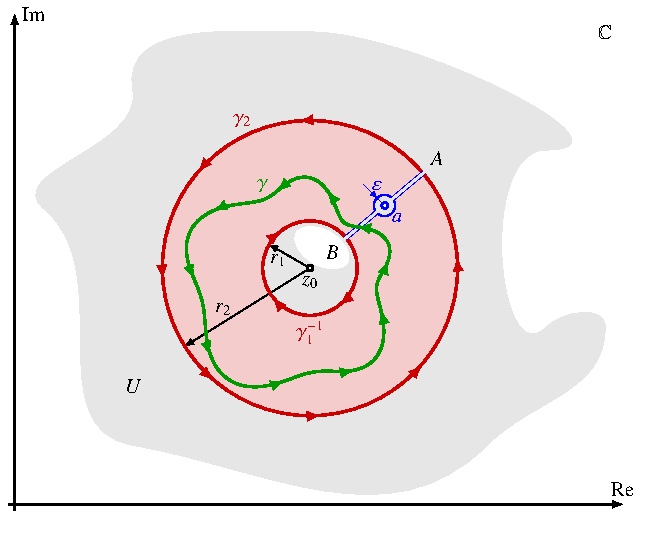
\includegraphics{chapters/040-analytisch/images/ring.pdf}
\caption{Die Funktion $f\colon U\to\mathbb{C}$ kann mithilfe eines
Pfadintegrals über den roten Rand berechnet werden, wodurch sich
die Entwicklung der Funktion in eine Laurent-Reihe finden lässt.
Die Koeffizienten der Laurent-Reihe können aber auch mit dem 
Weg $\gamma$ berechnet werden, der sich im Ringgebiet zu $\gamma_1$
oder $\gamma_2$ deformieren lässt.
\label{buch:analytisch:laurent:fig:ring}}
\end{figure}
